\subsection{NN Results}

\begin{figure}
% >> python3 paper_plots.py --NN -v --plots rec_vs_pred 
    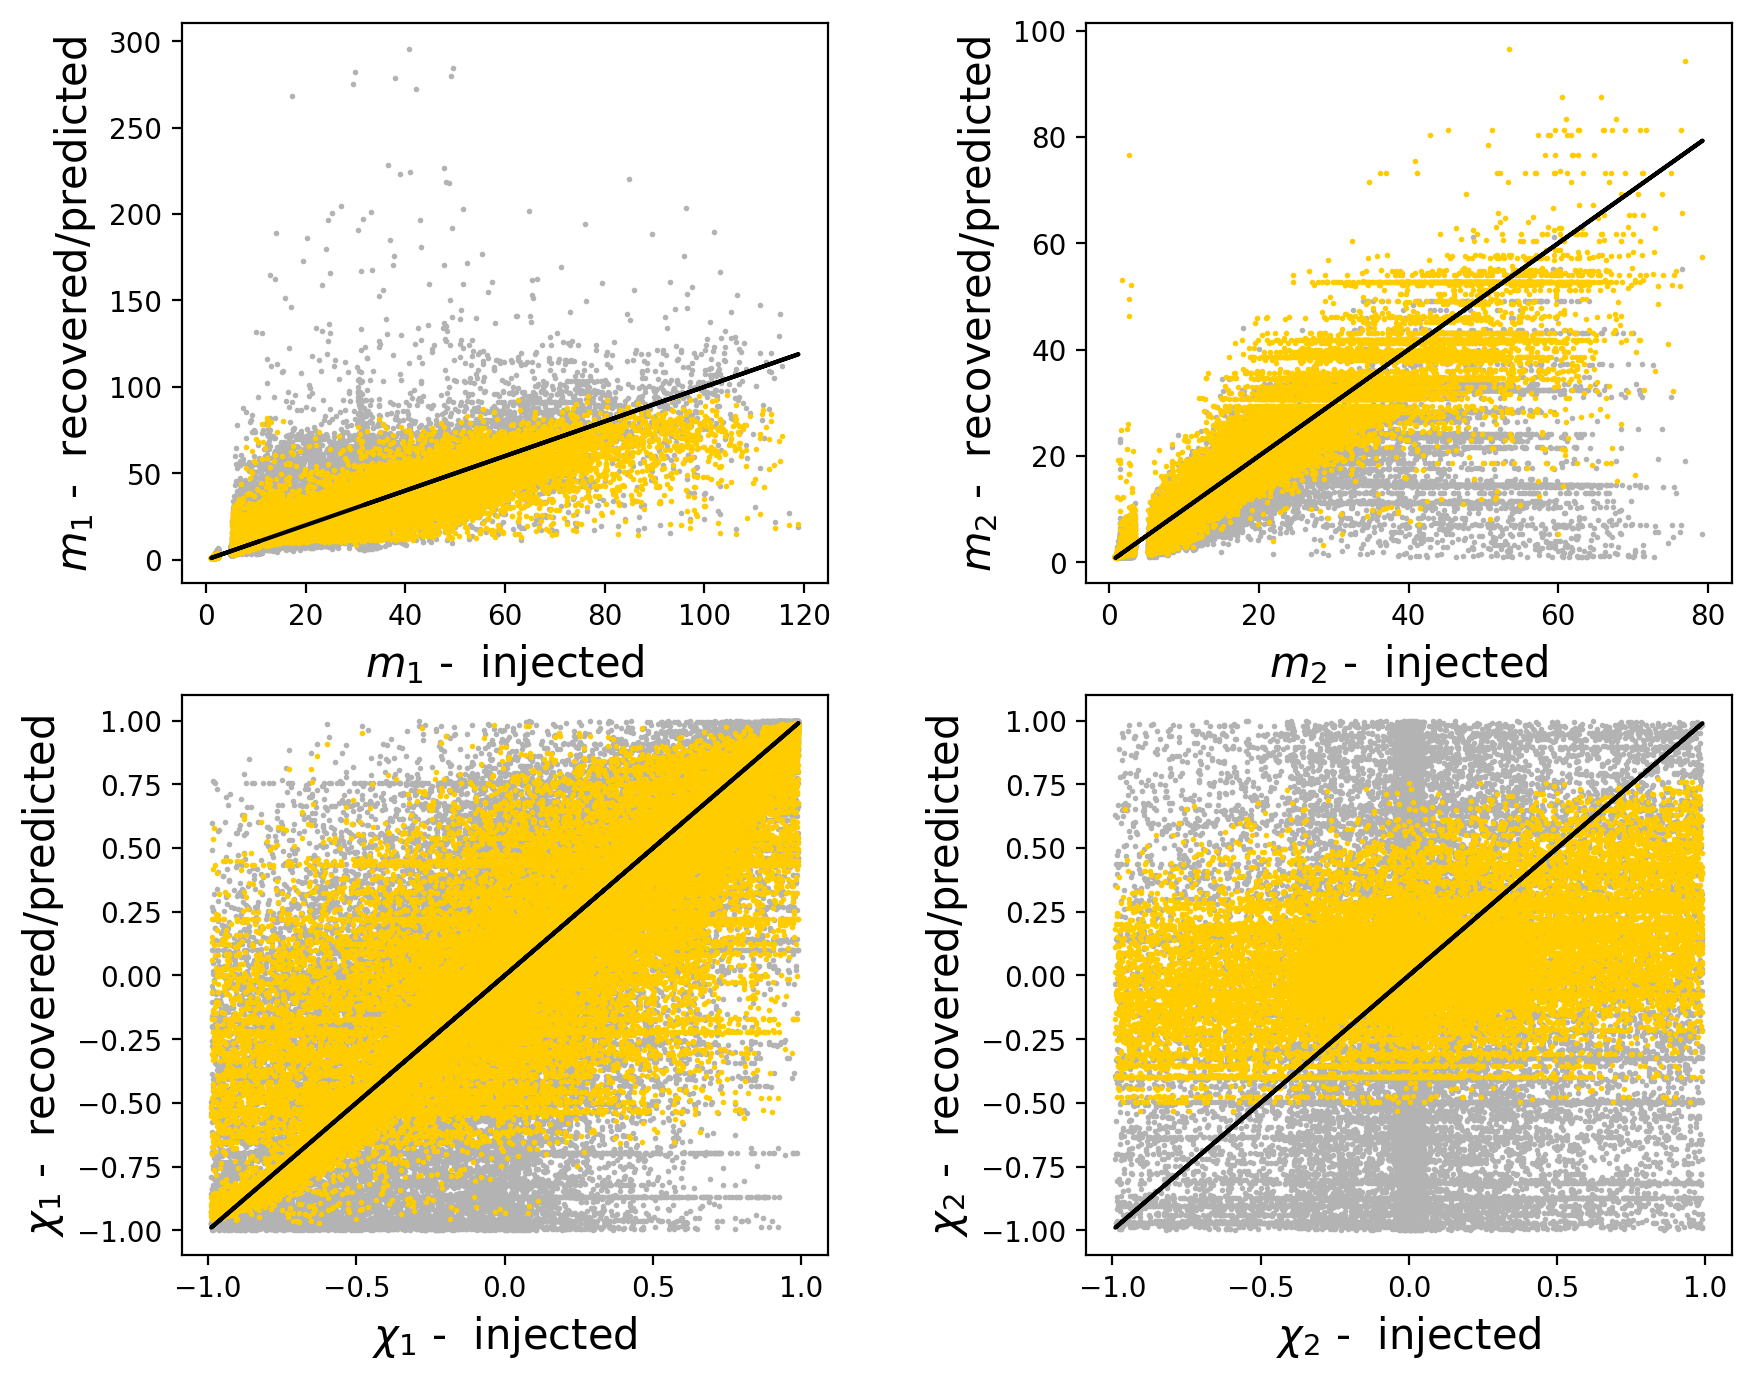
\includegraphics[width=0.45\textwidth]{m1m2chi1chi2_NN_recvspred.png}
    \caption{NN version of Fig.~\ref{m_chi_comparisons}}
        \label{m1m2chi1chi2_NN_recvspred}
\end{figure}

\begin{figure}
% >> python3 paper_plots.py --NN -v --plots histo --histo_logs 1 1 0 0 --histo_fmin -10 -10 -2 -2
    \centering
    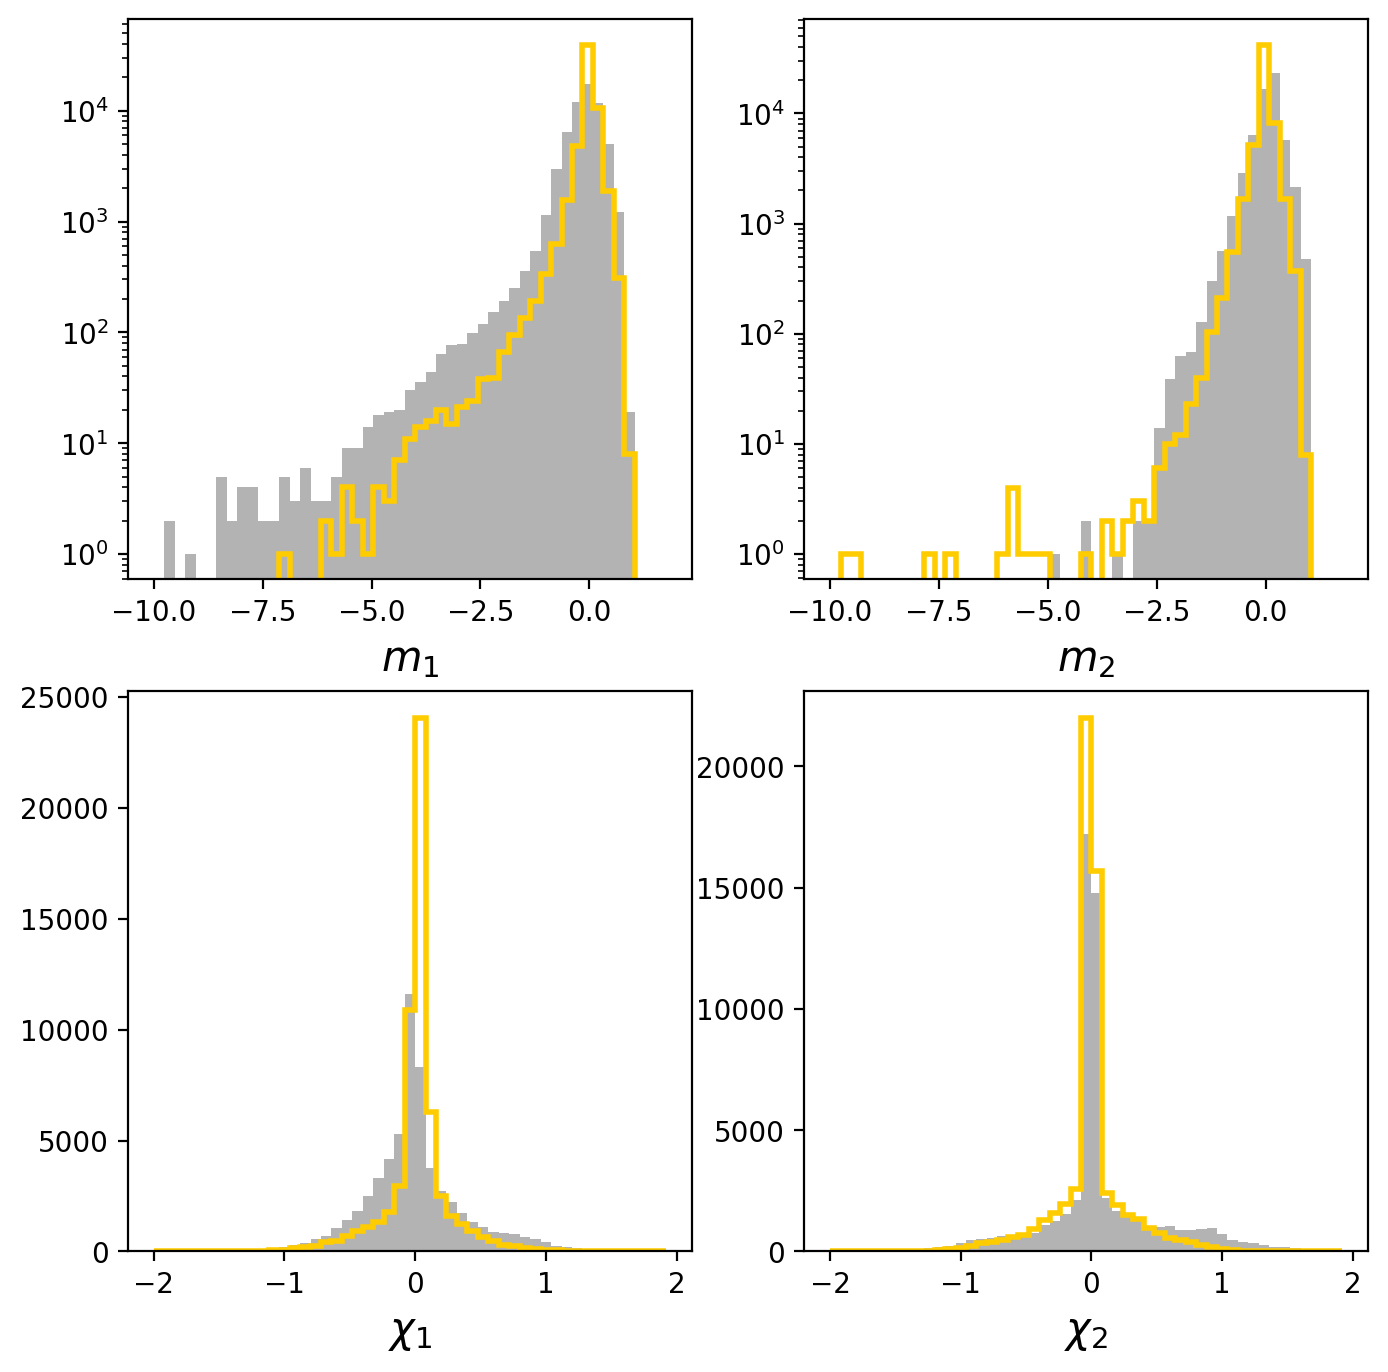
\includegraphics[width=0.45\textwidth]{m1m2chi1chi2_NN_histo.png}
    \caption{Histograms}
        \label{m1m2chi1chi2_NN_histo}
\end{figure}

\begin{table} 
% >> python3 paper_plots.py --NN -v --errortab --tab_format tex --vars m1m2chi1chi2
  \caption{\label{tab:NN_errors}  Mean differences in absolute value $|\Delta \bar{y}|=  \frac{1}{N} \Sigma |y^i_{\rm inj} - y^i_{\rm rec/pred}|$  
  and averages of the relative 
  differences in absolute value $|\delta \bar{y}| = \frac{1}{N} \Sigma \left( |y^i_{\rm inj} - y^i_{\rm rec/pred}|/y^i_{\rm inj} \right) $ for recovered and predicted data. 
  For spin variables, the standard deviation $\sigma_y$ is computed from the former, while for mass variables is computed from the latter. 
  Note that ${\cal{M}}_c$ is not predicted by the NN but it is computed from the predicted $m_i$.}
  \begin{center}
  \begin{tabular}{c|ccc|ccc}
  \hline\hline
  & $|\Delta \bar{y}_{\rm rec}|$  & $|\delta \bar{y}_{\rm rec}|$  & $\sigma_y^{\rm rec}$ & 
     $|\Delta \bar{y}_{\rm pred}|$ & $|\delta \bar{y}_{\rm pred}|$ & $\sigma_y^{\rm pred}$ \\
  \hline\hline
$m_1$          & $6.627$ & $0.348$ & $0.583$ & $3.534$ & $0.141$ & $0.310$ \\
$m_2$          & $2.827$ & $0.256$ & $0.362$ & $1.486$ & $0.127$ & $0.334$ \\
$\chi_1$       & $0.267$ &  /  & $0.389$ & $0.143$ &  /  & $0.240$ \\
$\chi_2$       & $0.274$ &  /  & $0.455$ & $0.151$ &  /  & $0.267$ \\
\hline
${\cal{M}}_c$  & $1.375$ & $0.040$ & $0.112$ & $0.786$ & $0.033$ & $0.089$ \\
  \hline\hline
\end{tabular}
\end{center}
\end{table}

\begin{table}
% >> python3 paper_plots.py --NN -v --errortab --tab_format tex --vars m1Mcchi1chi2
  \caption{\label{tab:NN_errors_temp} As Table~\ref{tab:NN_errors} but predicting $(m_1, {\cal{M}}_c, \chi_1, \chi_2)$. }
  \begin{center}
  \begin{tabular}{c|ccc|ccc}
  \hline\hline
 %& $\bar{|\Delta y_{\rm rec}|}$ & $\bar{|\Delta y_{\rm rec}/y|}$ & $\bar{|\sigma_y_{\rm rec}|}$ & & &  \\
  & $|\Delta \bar{y}_{\rm rec}|$  & $|\delta \bar{y}_{\rm rec}|$  & $\sigma_y^{\rm rec}$ & 
     $|\Delta \bar{y}_{\rm pred}|$ & $|\delta \bar{y}_{\rm pred}|$ & $\sigma_y^{\rm pred}$ \\
  \hline\hline
$m_1$          & $6.627$ & $0.348$ & $0.583$ & $3.572$ & $0.146$ & $0.311$ \\
${\cal{M}}_c$  & $1.375$ & $0.040$ & $0.112$ & $0.788$ & $0.036$ & $0.091$ \\
$\chi_1$       & $0.267$ &  /  & $0.389$ & $0.140$ &  /  & $0.241$ \\
$\chi_2$       & $0.274$ &  /  & $0.455$ & $0.151$ &  /  & $0.268$ \\
\hline
$m_2$          & $2.827$ & $0.256$ & $0.362$ & $1.509$ & $0.127$ & $0.342$ \\
  \hline\hline
\end{tabular}
\end{center}
\end{table}